\documentclass[a4]{beamer}
\usepackage{amssymb}
\usepackage{graphicx}
\usepackage{subfigure}
\usepackage{newlfont}
\usepackage{amsmath,amsthm,amsfonts}
%\usepackage{beamerthemesplit}
\usepackage{pgf,pgfarrows,pgfnodes,pgfautomata,pgfheaps,pgfshade}
\usepackage{mathptmx}  % Font Family
\usepackage{helvet}   % Font Family
\usepackage{color}

\mode<presentation> {
	\usetheme{Default} % was Frankfurt
	\useinnertheme{rounded}
	\useoutertheme{infolines}
	\usefonttheme{serif}
	%\usecolortheme{wolverine}
	% \usecolortheme{rose}
	\usefonttheme{structurebold}
}

\setbeamercovered{dynamic}

\title[MA4603/MA505]{Science Maths 3 \\ {\normalsize MA4704 Lecture 7B}}
\author[Kevin O'Brien]{Kevin O'Brien \\ {\scriptsize Kevin.obrien@ul.ie}}
\date{Autumn Semester 2016}
\institute[Maths \& Stats]{Dept. of Mathematics \& Statistics, \\ University \textit{of} Limerick}

\renewcommand{\arraystretch}{1.5}

\begin{document}
	
	\begin{frame}
		\titlepage
	\end{frame}
%==================================================%
	\begin{frame}
		\begin{figure}
\centering
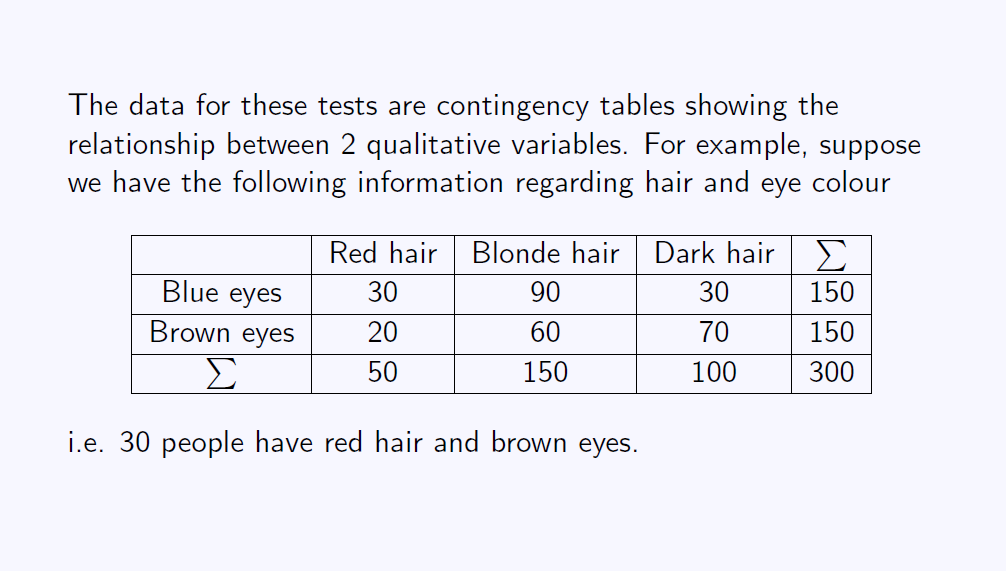
\includegraphics[width=1.1\linewidth]{ChiSquare1}
\end{figure}
	\end{frame}
%=========================================================%
%\begin{frame}
%		\begin{figure}
%			\centering
%			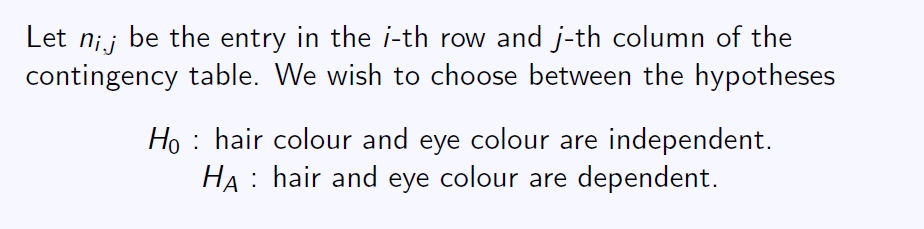
\includegraphics[width=1.1\linewidth]{ChiSquare2}
%
%		\end{figure}
%		
%	\end{frame}
%========================================================%
\begin{frame}
\frametitle{Chi Square Test For Independence}
\large
\noindent \textbf{Test for independence} \\ \bigskip
Let $n_{i,j}$ be the entry in the i-th row and j-th column of the
contingency table. We wish to choose between the hypotheses
\begin{description}
\item[H$_0$:] hair colour and eye colour are independent.
\item[H$_1$:] hair and eye colour are dependent.
\end{description}
%- 2 /25
\end{frame}
%========================================================%
\begin{frame}
\frametitle{Chi Square Test For Independence}
\large
\noindent \textbf{Row and column sums}
\begin{itemize}
\item The number of people in the sample with blue eyes is the sum of
the entries in the first row (150).
\item The number of people in the sample with brown eyes is the sum of
the entries in the second row (150).
\item The sum of all the entries is the number of individuals in the
sample (300).
\end{itemize}
%- 3 / 25
\end{frame}
%========================================================%
\begin{frame}
\frametitle{Chi Square Test For Independence}
\large
\begin{itemize}
	\item If the traits are independent, then the probability that an individual
	has a given hair colour and given eye colour is the product of the
	two corresponding probabilities e.g.
	\[\mbox{P(blond hair, blue eyes)} = \mbox{P(blond hair)}\times \mbox{P(blue eyes)}\]
	\item In order to test whether two traits are independent, we need to
	calculate what we would expect to observe if the traits were
	independent.
	\item The following calculations allow us to calculate what we expect to
	see under the null hypothesis of independence.
\end{itemize}

%- 6 / 25
\end{frame}
\end{document}
%========================================================%
\begin{frame}
\frametitle{Chi Square Test For Independence}
\large
\noindent \textbf{Expected number of observations in a cell under H0}\\
Under the null hypothesis, we expect ei ,j observations in cell (i , j ),
where
ei ,j = npi ,j
Hence, we can calculate the expected number of observations in
each cell
ei ,j = npi ,j =
ni ,•n•,j
n
,
i.e. the expected number is the row sum times the column sum
divided by the total number of observations.
%- Slide 9/25
\end{frame}
\begin{frame}
	\begin{figure}
\centering
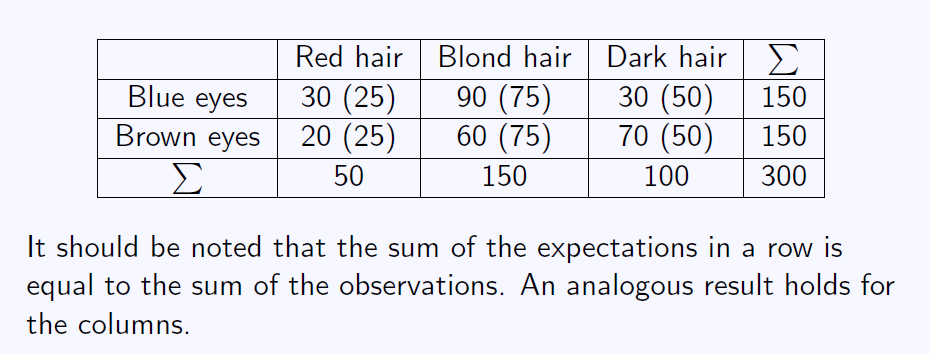
\includegraphics[width=0.7\linewidth]{ChiSquare11}
\caption{}
\label{fig:ChiSquare11}
\end{figure}

\end{frame}
%========================================================%
\begin{frame}
\frametitle{Chi Square Test For Independence}
\large
The test statistic is
T =
X
i ,j
(ni ,j - ei ,j )2
ei ,j
,
where the summation is carried out over all the cells of the
contingency table.
\begin{itemize}
\item The realisation of this statistic is labelled t. This is a measure of
the distance of our observations from those we expect under H0.
\item It should be noted that if the null hypothesis is true, then ni ,j and
ei ,j are likely to be similar, hence the realisation t will tend to be
close to 0 (by definition this realisation is non-negative). Large
values of t indicate that the traits are dependent.
\end{itemize}
%- 12 / 25
\end{frame}
%===========================================================%
\begin{frame}
	\begin{figure}
		\centering
		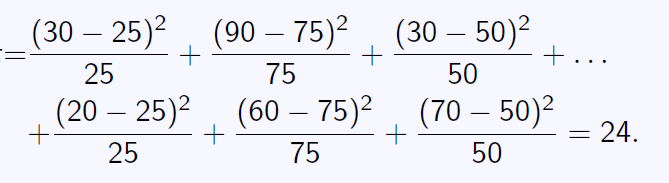
\includegraphics[width=0.7\linewidth]{ChiSquare13}
		\caption{}
		\label{fig:ChiSquare13}
	\end{figure}
	
\end{frame}
%========================================================%
\begin{frame}
\frametitle{Chi Square Test For Independence}
\large

Distribution of the test statistic under H0
\begin{itemize}
\item Given the traits are independent, the test statistic has an
approximate chi-squared distribution with $(r - 1) \times (c - 1)$ degrees
of freedom, where r and c are the numbers of rows and columns,
respectively.
\item It should be noted that this approximation is reasonable if at
least 5 observations are expected in each cell under H0.
\end{itemize}
% - 14/25

\end{frame}
%========================================================%
\begin{frame}
\frametitle{Chi Square Test For Independence}
\large
\noindent \textbf{Making conclusions}
\begin{itemize}
	\item Since large values of t indicate that the traits are dependent, we
	reject the null hypothesis of independence at a significance level of
	if
	t > 2(
	r-1)(c-1),,
	where 2(
	r-1)(c-1), is the critical value for the appropriate
	chi-squared distribution. 
	
\item These values can be read from Table 8.
\end{itemize}


% - 15 / 25
\end{frame}
%========================================================%
\begin{frame}
\frametitle{Chi Square Test For Independence}
\large
Describing the nature of an association
\begin{itemize}
\item In order to see the nature of the association between hair and eye
colour, we should compare the observed and expected values.
\item Comparing the table of observed and expected values, it can be
seen that dark hair is associated with brown eyes and blond hair
with blue eyes (in both cases there are more observations than
expected under the null hypothesis).
\end{itemize}
% - 17 / 25

\end{frame}
%========================================================%
\begin{frame}
\frametitle{Chi Square Test For Independence}
\large
\noindent \textbf{Simpsons Paradox}
\begin{itemize}
\item The nature of an association between two traits may change and
even reverse direction when the data from several groups is
combined into a single group.
For example, consider the following data regarding admissions to a
university.
\item The Physics department accepted 60 applications from 100 males
and 20 applications from 30 females.
\item The Fine Arts department accepted 10 applications from 100
males and 30 applications from 170 females.
\end{itemize}
%- 18/25

\end{frame}
%========================================================%
\begin{frame}
\frametitle{Chi Square Test For Independence}
\large
\noindent \textbf{Simpsons Paradox}
\begin{itemize}
\item Hence, the Physics department accepted 60\% of applications from
males and 66.7\% of applications from females. 
\item The Fine Arts
department accepted 10\% of applications from males and 17.6\% of
applications from females.
\item Hence, in both departments females are slightly more successful.
\end{itemize}
%- 19/25
\end{frame}
%========================================================%
\begin{frame}
\frametitle{Chi Square Test For Independence}
\large
\noindent \textbf{Simpsons Paradox}
\begin{itemize}
\item Combining the departments, we obtain the following contingency
\item Combining the results females are less successful.
\item We now test the null hypothesis that acceptance is independent of
sex. 
\item The alternative is that acceptance is associated with sex (i.e.
the likelihood of acceptance depends on sex).
\end{itemize}
%- 20/25

\end{frame}
%========================================================%
\begin{frame}
\frametitle{Chi Square Test For Independence}
\large
Testing the null hypothesis at the 5\% level, the critical value is
$\chi^2_{(
r-1)(c-1),)}$ = $\chi^2_{(1,0.05)}$ = 3.841.
Since t > $\chi^2_{(1,0.05)}$ = 3.841, we reject the null hypothesis.
\begin{itemize}
\item We conclude that acceptance is associated with sex. Looking at
the table which compares the observed and expected values,
females are less likely to be accepted than expected.
\item Hence, using this data we might conclude that there is evidence
that females are discriminated against.
\end{itemize}
%- Slide 23 / 25
\end{frame}
%========================================================%
\begin{frame}
\frametitle{Chi Square Test For Independence}
\large
\begin{itemize}
\item However, in both departments a female is more likely to be
accepted.
\item On average, females are less likely to be accepted since they are
more likely to apply to the fine arts department and the fine arts
department rejects a higher proportion of applications.
\end{itemize}
%%- 24
\end{frame}
%========================================================%
\begin{frame}
\frametitle{Chi Square Test For Independence}
\large
\noindent \textbf{Lurking variables}
In this case department is what we call a hidden or lurking variable.
A hidden or lurking variable is a variable which may influence the
observed results, but is not considered in the analysis.
For example, women’s salaries are significantly lower on average
that men’s salaries.
\begin{enumerate}
\item Can this be used as evidence that women are
discriminated against?
\item What are the lurking variables which may explain
such a difference?
\item How should we test whether females are
discriminated against with regard to salary?
\end{enumerate}
%%25 / 25
\end{frame}
\end{document}